\documentclass[10pt,journal,compsoc]{IEEEtran}
% * <carlos.segarra@bsc.es> 2017-09-21T09:08:41.072Z:
%
% ^.

\ifCLASSOPTIONcompsoc
  % IEEE Computer Society needs nocompress option
  % requires cite.sty v4.0 or later (November 2003)
  \usepackage[nocompress]{cite}
\else
  % normal IEEE
  \usepackage{cite}
\fi
\usepackage[pdftex]{graphicx}
\usepackage{amsmath}
\newtheorem{definition}{Definition}
\interdisplaylinepenalty=2500
%\usepackage{algorithmic}
\usepackage{array}
\ifCLASSOPTIONcompsoc 			     	 \usepackage[caption=false,font=footnotesize,labelfont=sf,textfont=sf]{subfig}
\else
  \usepackage[caption=false,font=footnotesize]{subfig}
\fi
\ifCLASSOPTIONcaptionsoff
  \usepackage[nomarkers]{endfloat}
 \let\MYoriglatexcaption\caption
 \renewcommand{\caption}[2][\relax]{\MYoriglatexcaption[#2]{#2}}
\fi
\usepackage{url}
\hyphenation{op-tical net-works semi-conduc-tor}

\usepackage{algorithm}% http://ctan.org/pkg/algorithms
\usepackage{algpseudocode}% http://ctan.org/pkg/algorithmicx

%URL
\usepackage{hyperref}
\usepackage{tabularx}

%Plotting
\usepackage{tikz}
\usetikzlibrary{patterns}
%\usepackage{tikz-3dplot} 
\usepackage{pgfplots}

\usepackage{varwidth}% http://ctan.org/pkg/varwidth

%Code snippets
\usepackage{xcolor}
\usepackage{listings}
\definecolor{codegreen}{rgb}{0,0.6,0}
\definecolor{codegray}{rgb}{0.5,0.5,0.5}
\definecolor{codepurple}{rgb}{0.58,0,0.82}
\definecolor{backcolour}{rgb}{0.98,0.98,0.95}
\lstdefinestyle{mystyle}{
    backgroundcolor=\color{backcolour},   
    commentstyle=\color{codegreen},
    keywordstyle=\color{magenta},
    numberstyle=\tiny\color{codegray},
    stringstyle=\color{codepurple},
    basicstyle=\footnotesize\ttfamily,breaklines=true,
    breakatwhitespace=false, 
    xleftmargin=20pt, 
    xrightmargin=20pt,       
    breaklines=true,                 
    captionpos=b,                    
    keepspaces=true,                 
    numbers=left,                    
    numbersep=5pt,                  
    showspaces=false,                
    showstringspaces=false,
    showtabs=false,                  
    tabsize=2,
    framextopmargin=50pt,
    frame=bottomline,
    basicstyle=\footnotesize\ttfamily,
    language=Python
}
\lstset{literate=
  {á}{{\'a}}1 {é}{{\'e}}1 {í}{{\'i}}1 {ó}{{\'o}}1 {ú}{{\'u}}1
  {Á}{{\'A}}1 {É}{{\'E}}1 {Í}{{\'I}}1 {Ó}{{\'O}}1 {Ú}{{\'U}}1
  {à}{{\`a}}1 {è}{{\`e}}1 {ì}{{\`i}}1 {ò}{{\`o}}1 {ù}{{\`u}}1
  {À}{{\`A}}1 {È}{{\'E}}1 {Ì}{{\`I}}1 {Ò}{{\`O}}1 {Ù}{{\`U}}1
  {ä}{{\"a}}1 {ë}{{\"e}}1 {ï}{{\"i}}1 {ö}{{\"o}}1 {ü}{{\"u}}1
  {Ä}{{\"A}}1 {Ë}{{\"E}}1 {Ï}{{\"I}}1 {Ö}{{\"O}}1 {Ü}{{\"U}}1
  {â}{{\^a}}1 {ê}{{\^e}}1 {î}{{\^i}}1 {ô}{{\^o}}1 {û}{{\^u}}1
  {Â}{{\^A}}1 {Ê}{{\^E}}1 {Î}{{\^I}}1 {Ô}{{\^O}}1 {Û}{{\^U}}1
  {œ}{{\oe}}1 {Œ}{{\OE}}1 {æ}{{\ae}}1 {Æ}{{\AE}}1 {ß}{{\ss}}1
  {ű}{{\H{u}}}1 {Ű}{{\H{U}}}1 {ő}{{\H{o}}}1 {Ő}{{\H{O}}}1
  {ç}{{\c c}}1 {Ç}{{\c C}}1 {ø}{{\o}}1 {å}{{\r a}}1 {Å}{{\r A}}1
  {€}{{\euro}}1 {£}{{\pounds}}1 {«}{{\guillemotleft}}1
  {»}{{\guillemotright}}1 {ñ}{{\~n}}1 {Ñ}{{\~N}}1 {¿}{{?`}}1
}
\lstset{style=mystyle}
%\pgfplotsset{compat=1.14}

\begin{document}

\title{TB-DBSCAN: Task Based - DBSCAN\\ \LARGE{An implementation using the PyCOMPSs framework}}

\author{Carlos~Segarra \\ 
\href{mailto:carlos.segarra@bsc.es}{carlos.segarra@bsc.es}}

\IEEEtitleabstractindextext{%
\begin{abstract}
% Abstract structure:
% - Introduce the importance of the topic and the scope. DONE
% - Describe very briefly what has been done (general description without details). DONE
% - Give a global overview of the achievements. DONE
% - REVIEW: 

The DBSCAN algorithm is one of the most popular clustering techniques used nowadays. However there is a lack of distributed implementations. Additionally, parallel implementations fail when they try to scale to hundreds of cores. The scope of this report is to provide a novel implementation of the algorithm that behaves well in large distributed architectures and with big datasets. Using the PyCOMPSs framework and testing on the Mare Nostrum 4 supercomputer, encouraging results have been obtained reaching a 2467 speedup when run with 4096 cores. Everything whilst keeping the code clean and transparent to the user.
\end{abstract}

\begin{IEEEkeywords}
DBSCAN, Clustering, Machine Learning, Distributed Computing, COMPSs, PyCOMPSs
\end{IEEEkeywords}}
\maketitle
\IEEEdisplaynontitleabstractindextext
\IEEEpeerreviewmaketitle

\IEEEraisesectionheading{\section{Introduction}\label{sec:introduction}}

% Introduction structure {
% - Introduce the topic and the scope (give a use case can be helpful). DONE
% - Brief overview of DBSCAN (what is it used for?) DONE
% - Purpose of the article. * DONE
% - Motivation and objective/s. * ??
% - Contribution of the paper. * DONE
% - Define the structure of the article DONE
%   * These points can be in another order.

Big data and data mining is on the daily agenda of nowadays' engineers and having tools to process and analyze this data quickly is of vital importance. Precisely, machine learning, and more precisely, unsupervised learning and clustering are useful for detecting trends and patterns between data without needing the user to previously classify it. The DBSCAN belongs to this family of methods and is useful for detecting non-convex without having to guess the number of clusters.

TB-DBSCAN (Task Based - DBSCAN) is the first implementation of the DBSCAN clustering algorithm within the \cite{compss} framework for distributed computing. The main scope of this paper is to implement a task based version of the algorithm in Python with the PyCOMPSs syntax, test it in high-stress, highly distributed architectures and scale to hundreds of cores.

Which is the main contribution of this paper? Wait until results.

Section \ref{sec:related_work} covers related work, other attempts to implementing a parallel version of the DBSCAN in other programming frameworks as well as other clustering algorithms. It briefly covers different benchmarks related to performance and emphasises the novelty of our proposal. Following along, Section \ref{sec:background} introduces the state of the art of clustering algorithms, describes the Density-Based Spatial Clustering Algorithm the programming model chosen for the implementation and covers the environment where tests have been performed. Section \ref{sec:implementation} describes the algorithm developed to fulfill the scope of the paper, the dependency graph drawn by it and covers possible equivalence issues faced when reinterpreting a sequential algorithm as a parallel one. Section \ref{sec:performance} summarizes all the tests performed with synthetic and real data, presents the results and gives a critical review to the algorithm using post-mortem analysis tools and tracing. Lastly Section \ref{sec:conclusion} gathers the conclusions obtained and proposes further developments that did not fit our initial scope.
% }

\section{Related Work} \label{sec:related_work}

Quickly after the algorithm was first presented (1996) the necessity to feed the clustering algorithm with big datasets arose. First approaches of DBSCAN parallelization only dealt with the region query issue which is indeed where more calculus power is invested. For instance, \cite{related_1} presents a skeleton-structured program where slaves are responsible for answering the regions query performed by the master.

Latter developments started including smart data partitioning. \cite{related_2} proposes what has become a standard procedure for distributed implementations of the DBSCAN. Initially data is efficiently divided, secondly a series of partial clusterings are performed and final results are merged by the master. Most implementations differ on both the partition and the merging. \cite{related_2} divides data using a low-precision hierarchical clustering algorithm and merges the data using a graph connectivity technique similar to the one used in this paper. Graph connectivity techniques are also used in \cite{related_4}. Yaobin HE et. al \cite{related_3} propose a novel partitioning method based on computational costs predictions and merge results using a 4 step MapReduce strategy. 

Latest developments focus on flexibility and scalability to high feature datasets. A. Lulli \cite{related_5} presents a Spark-based algorithm that does not require euclidean metric and that works with arbitrary data.

The novelty of our proposal lies that in all the previously mentioned papers, the code might be quite difficult to understand and specially to mantain for a user. Taking advantage of the COMPSs framework for distributed programming, the final code produced is highly-readable.
% Add related works (publications) with the same or similar objective (even for another clustering algorithms or frameworks). DONE

% Don't forget to point out the differences between other proposals and the one presented in the paper. DONE 
% I would try to concentrate the main difference/novelty as the last phrase of this section to remark what makes this work innovative compared to others. DONE




%%%%%%%%%%%%%%%%%%%%%%%%%%%%%%%%%%%%%%%%%%%%%%%%%%%%%%%%%%%%
%%%%%%%%%%%%%%%%%%     BACKGROUND       %%%%%%%%%%%%%%%%%%%%
%%%%%%%%%%%%%%%%%%%%%%%%%%%%%%%%%%%%%%%%%%%%%%%%%%%%%%%%%%%%


\section{Background} \label{sec:background}

% JC: This section can be used to provide the necessary background for understanding the following sections.
% JC: Here, DBSCAN can be defined formally, as well as PyCOMPSs.

Clustering algorithms aim to infer the hidden pattern underlying a non-classified dataset. The DBSCAN is a density based clustering algorithm introduced in Subsection \ref{sub-sec:the-algorithm}

This section provides the necessary information to firstly understand the implementation proposed and secondly contextualise the tests performed.

\subsection{The algorithm: DBSCAN} \label{sub-sec:the-algorithm}

% Formal definition of DBSCAN

The \textbf{D}ensity-\textbf{B}ased \textbf{S}patial \textbf{C}lustering \textbf{A}lgorithm with \textbf{N}oise (\textbf{DBSCAN}) is a clustering algorithm based on point density. It was proposed in 1996 \cite{original-paper} and has become one of the reference techniques for non-supervised learning. To take a first dive into the implementation, a few previous definitions are mandatory.

\begin{definition}
The $\varepsilon$\textbf{-neighbourhood} of a point $p$ from a dataset $D$ and given a distance $d$ is
$$N_{\varepsilon}(p) = \lbrace q \in D: d(p,q) < \varepsilon \rbrace$$ 
\end{definition}

The general approach partitions the set of points in three subsets:
\begin{definition}
\begin{itemize}
\item A point $p$ is said to be \textbf{\textit{core point}} if it has over \textit{minPoints} neighbours within its $\varepsilon$-neighbourhood.
\item A point $p$ is said to be \textbf{\textit{reachable}} if it lies within a $\varepsilon$-neighbourhood of a core point in spite of not being one.
\item A point $p$ is said to be \textbf{\textit{noise}} if it does not fulfil any of the previous definitions.
\end{itemize}
\end{definition}

\begin{definition}
A \textbf{Cluster} $C$ is a subset of a dataset $D$ such that for all $p \in C$:
\begin{itemize}
\item[(i)] $p$ is a core-point or reachable
\item[(ii)] $\forall p,q \in C, \exists p_1, \ldots,  p_r$ fulfilling (i) such that $p \in N_{\varepsilon}(p_1)$, $p_i \in N_{\varepsilon}(p_{i+1})$ and $p_r \in N_{\varepsilon}(q)$ where only, maybe $p$ and/or $q$ are reachable
\end{itemize}
\end{definition}

\begin{definition} \label{dist-definition}
The \textbf{distance between sets} $A$ and $B$ given a metric d is
$$d(A,B)=\min \lbrace d(a,b): a \in A, b \in B \rbrace$$
\end{definition}

In Algorithm \ref{alg:original-main} we present a schematic pseudocode of the original algorithm. For each new point being processed that has not been processed yet, we detect wether it is a core point or not. If it is, we stack all his neighbours and process them if they have not been processed yet. If one of these neighbours is a core point, all his neighbours are stacked on top of the previous. If the original point is not a core point, it is labeled as noise.


\begin{algorithm}
  \caption{Schematic Implementation of the DBSCAN algorithm. \label{alg:original-main}}
  \begin{algorithmic}[1]
    \Function{DBSCAN}{$data$, $epsilon$, $min\_points$}
        \State $next\_ID \gets FIRST\_ID$
        \ForAll{$point$ \textbf{ in } $data$}
            \If{$point$ \textbf{ is } $core\_point$}
                \State $\text{label}(point)$
                \State $point\_stack.\text{add}(\text{neigh}(point))$
                \ForAll{$n\_point$ \textbf{ in } $point\_stack$}
                    \If{$n\_point$ \textbf{ is } $core\_point$}
                        \State $point\_stack.\text{add}(\text{neigh}(n\_point))$
                    \EndIf
                    \State $\text{label}(n\_point)$
                \EndFor
            \EndIf
        \EndFor
    \EndFunction
  \end{algorithmic}
\end{algorithm}

\subsubsection{Other Clustering Algorithms} \label{sec:other-clust-alg}

% JC: I like this subsubsection, since it focuses on the difference with other clustering algorithms rather than being a related work, and helps to understand DBSCAN.
The urge to process larger and larger amounts of data without knowing their structure nor the underlying pattern puts clustering techniques in the limelight of machine learning algorithms. General purpose classifiactions difference between: hierarchical, centroid-based, distribution based and density based clustering.

Recently a lot of research has been dedicated to improving clustering algorithms, resulting in the current classification in four different categories: hierarchical clustering, centroid-based clustering, distribution-based clustering and density based clustering.

In comparison to its main competitor the \textbf{k-means} algorithm \cite{kmeans}, DBSCAN is robust to outliers, it does not require an initial guess of the number of clusters and it is able to detect non-convex clusters as exposed in Figure. To obtain the Figure the dataset has been generated using the \textit{Sklearn} package for datasets (\href{http://scikit-learn.org/stable/modules/generated/sklearn.datasets.make_moons.html}{\texttt{make\_moons}}), the DBSCAN algorithm is the one presented in this document and the k-means is a personal implementation available on the \href{https://github.com/csegarragonz/DBSCAN-pyCOMPSs}{project's GitHub repository}.

\subsubsection{S.o.A for sequential and distributed implementations}

% JC: I also like this subsection. 

There are a variety of implementations of the DBSCAN raging from the more naive ones to more complex ones. As for comparison, a naive implementation following the exact guidelines of \cite{ReferencePaper} can be found \href{https://github.com/csegarragonz/DBSCAN-pyCOMPSs/blob/master/ext_versions/DBSCAN_Seq.py}{here}. One of the most extended and used versions programmed in \texttt{Python} is the one by \href{http://scikit-learn.org/stable/modules/generated/sklearn.cluster.DBSCAN.html}{Sklearn}.

When it comes to distributed implementations of the algorithm, most of them can be summarized in applying an efficient DBSCAN to a chunk of the dataset and using some sort of synchronization or MapReduce. Otherwise, the DBSCAN for PyCOMPSs reformulates the algorithm trying to adapt it to distributed architectures making sure it is still equivalent to the original implementation.

\subsection{The framework: COMPSs} \label{subec:compss_framework}

% COMPSs/PyCOMPSs definition

The \href{https://www.bsc.es/research-and-development/software-and-apps/software-list/comp-superscalar}{COMPSs} framework\cite{compss} is a programming model designed to ease the development of applications for distributed architectures. The user programs a sequential code and defines the so-called \texttt{tasks}. The COMPSs runtime infers the dependencies and schedules the executions basing on the resources available. The model is developed in Java but has bindings for both \texttt{C} and \texttt{Python}. \texttt{PyCOMPSs}\cite{pycompss} is the model chosen to develop the application. A master orchestrates a series of workes with a certain number of threads that are responsible of running tasks. In order to mark a function as a task for the scheduler to take it into account, a small decorator must be added. For remote objects to be available at the master thread a synchronisation is ran using the \texttt{compss\_wait\_on} built-in method. \texttt{COMPSs} is complemented by a set of tools for facilitating the monitoring and the post-mortem performance analysis (see Section ).

% \begin{figure}
% \animategraphics[autoplay,controls,loop,scale=1]{3}{img/anim-}{0.png}{4.png}
% \end{figure}

%%%%%%%%%%%%%%%%%%%%%%%%%%%%%%%%%%%%%%%%%%%%%%%%%%%%%%%%%%%%
%%%%%%%%%%%%%%%%%%%     PROPOSAL       %%%%%%%%%%%%%%%%%%%%%
%%%%%%%%%%%%%%%%%%%%%%%%%%%%%%%%%%%%%%%%%%%%%%%%%%%%%%%%%%%%

\section{Implementation Proposal} \label{sec:implementation}

In this section, we describe our distributed, task-based DBSCAN algorithm (TB-DBSCAN), which is completely equivalent to the original implementation \cite{ReferencePaper}. The code is public and can be found in the project's GitHub Repository\footnote{https://github.com/csegarragonz/DBSCAN-pyCOMPSs}. TB-DBSCAN takes three input arguments: \texttt{data\_file}, \texttt{min\_points} and \texttt{$\varepsilon$}, and outputs a data file with the clustered data.

\begin{algorithm}
  \caption{Main method of the TB-DBSCAN algorithm. \label{alg:main}}
  \begin{algorithmic}[1]
    \Function{DBSCAN}{$data\_file$, $epsilon$, $min\_points$}
        \ForAll{$square$ \textbf{in} $data\_file$}
            \State $frag\_data \gets \text{load\_data}(data\_file)$
            \State $local\_clusters \gets \text{partial\_scan}(frag\_data)$
            \State $cluster\_map \gets \text{sync\_clusters}(local\_clusters)$
        \EndFor
        \State $frag\_data \gets \text{compss\_wait\_on}(frag\_data)$
        \State $ maps \gets \text{map\_clusters} (frag\_data, cluster\_map)$
        \ForAll{$square$ \textbf{in} $frag\_data$}
            \State $\text{expand\_clusters} (square, maps)$
        \EndFor
        \State $\textbf{return} \hspace{5pt} 1$
    \EndFunction
  \end{algorithmic}
\end{algorithm}

Algorithm \ref{alg:main} drafts a general overview of TB-DBSCAN. Initially, TB-DBSCAN organises the input data in an $n$-dimensional space ($D$) where $n$ is the number of features of each point. $D$ is chunked in different regions ($R_i$) stored in independent data files. For each region, TB-DBSCAN retrieves core points and looks for local clusters (line 4). Then, TB-DBSCAN looks for possible cluster relations within a square and it's neighbours. Lastly it combines all the data gathered, updates the local labels and adds non-core points to the clusters (lines 7, 8 and 9).

In the following subsections we describe the different task methods in detail.

\subsection{Task 1: Data Loading} \label{subsec:data-loading}

The \texttt{load\_data} task method loads a chunk of a region($R_i$) to memory and initialises the points as noise (not belonging to any cluster).

We assume that each feature of each point in the dataset is normalised to the $[0,1]$ interval and that it is divided in different files, each one corresponding to a region $R_i \subset D$. For instance, if the points are two-dimensional, a possible file distribution would consist of the following files: \texttt{data\_0\_0.txt}, \texttt{data\_0\_1.txt}, \dots, \texttt{data\_0\_9.txt}, \texttt{data\_1\_0.txt}, \dots, \texttt{data\_9\_9.txt}. A point $p$ belongs to a certain file $R_i$ if the first decimal position of each feature matches the two numbers in the file name. I.e $p \in \texttt{data\_i\_j.txt} \Leftrightarrow p = [0.i\dots, 0.j\dots]$. This spatial file distribution enables us to efficently query the neighbours of a point without needing a complex data structure.

Since the size of these files can be arbitrarily big, one task only load one chunk of the file into memory at a time. For this, we employ a \emph{recursive scheme} to spawn a variable number of tasks, guaranteeing that each task does not process more than a fixed number of data points. This \emph{recursive scheme} can be seen in Algorithm \ref{alg:rec-approach}.

\begin{algorithm}
  \caption{Limit the number of points processed by a particular task. \label{alg:rec-approach}}
  \begin{algorithmic}[1]
    \Function{orquestrate\_task}{$data\_file, q=1, r=0$}
        \State $THRESHOLD = TH\_VALUE$
            \If{$\text{len}(data\_file)/q \geq TH\_VALUE$}
                \State $out = \text{orquestrate\_task}(data\_file, 2*q, 2*r + 0)$
                \State $out = \text{orquestrate\_task}(data\_file, 2*q, 2*r + 1)$
            \Else
                \State $out.append(\text{task}(data\_file, q, r))$
            \EndIf
        \State \textbf{return} $out$
    \EndFunction
  \end{algorithmic}
\end{algorithm}

The \texttt{orquestrate\_task} function takes three input parameters, a path to a data file ($DF$) whose length is known, a quotient $q$ initially set to 1 and a remainder $r$ initially set to $0$. If $q$ divides the data file in chunks larger than a threshold value, two more \texttt{orquestrate\_task} methods are invoked (lines 3-5). Otherwise a task is spawned which will process all the points in $DF$ whose index ($p_1, p_2, \dots$) is congruent with $r$ modulo $q$ (line 7). All the outputs are lastly gathered to reduce the different results obtained from the different tasks applied to the different chunks from $DF$.

\subsection{Task 2: Partial Scan} \label{sec:partial-scan}
The \texttt{partial\_scan} task method identifies and clusters the core points (i.e points with more than \texttt{min\_points} neighbours) in a region.

Given a space region $R_i$ let us define the neighbour regions of $R_i$, $NR(R\_i)$ as the set of regions reachable from $R_i$ with $\varepsilon$ distance. This is,
$$ NR(R_i) = \lbrace R_j \subset D \text{ : } d(R_i, R_j) \rbrace $$
where $d$ is the infinity norm distance. We choose this metric to take advantage of our file distribution (see figure \ref{fig:neigh-loc}).

\begin{figure}[!ht]
\centering
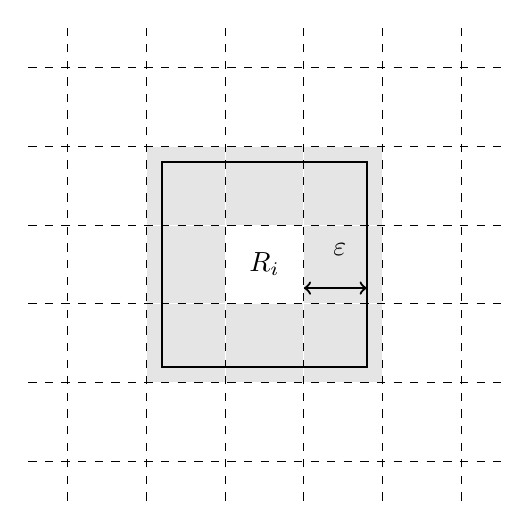
\begin{tikzpicture}[every node/.style={minimum size=1cm-\pgflinewidth, outer sep=0pt}]
    \node at (0.5, 0.5) {$R_i$};
    \node[fill=gray!20] at (1.5, 1.5) {};
    \node[fill=gray!20] at (-0.5, 1.5) {};
    \node[fill=gray!20] at (0.5, 1.5) {};
    \node[fill=gray!20] at (0.5, -0.5) {};
    \node[fill=gray!20] at (-0.5, 0.5) {};
    \node[fill=gray!20] at (-0.5, -0.5) {};
    \node[fill=gray!20] at (1.5, 0.5) {};
    \node[fill=gray!20] at (1.5, -0.5) {};
    \draw[step=1cm, color=black, dashed] (-2.5,-2.5) grid (3.5,3.5);

    \draw[<->, thick, black] (1, 0.2) -- (1.8, 0.2) node[midway, above] {\vspace{-5pt} $\varepsilon$};
    \draw[thick, black] (-0.8, -0.8) rectangle (1.8, 1.8);
\end{tikzpicture}
\caption{$R_i$ surrounded by $NR(R_i)$ coloured in gray and further regions left white. \label{fig:neigh-loc}}
\end{figure}

\emph{Applying the recursive scheme to $R_i$} each task looks for core points in a chunk of $R_i$ considering all the points in $NR(R_i)$. We have chosen to fraction $R_i$ rather than $NR(R_i)$ to guarantee the sufficiency of the results with no additional effort. I.e, dividing $NR(R_i)$ could lead to a task finding $\frac{min\_points}{2}$ neighbours of a given point and another one finding other $\frac{min\_points}{2}$ of the same point, missclassifying it as non-core when it really is.

The partial scan method labels each point $p$ according to the following three rules:
\begin{itemize}
    \item[(i)] If $| N_{\varepsilon} (p) | \geq \texttt{min\_points}$ we label it as a core point.
    \item[(ii)] If $| N_{\varepsilon} (p) | < \texttt{min\_points}$ but $ \exists q \in  N_{\varepsilon} (p) $ such that $ | N_{\varepsilon} (q) | \geq \texttt{min\_points}$ then TB-DBSCAN labels $p$ in a way that remembers to copy $q$'s id when the clustering is finished.
    \item[(iii)] The point is not a core point neither has one in it's $\varepsilon$-neighbourhood. TB-DBSCAN keeps the original label but keeps track of $p$'s neighbours.
\end{itemize}
We consider cases (ii) and (iii) to reduce the computational cost of labeling reachable points.

% \begin{figure}[!h]
% \centering
% \begin{tikzpicture}[every node/.style={minimum size=1cm-\pgflinewidth, outer sep=0pt}]
%     % Graphic area
%     \draw[step=1cm, color=black, dashed] (-1.25,-1.25) grid (2.25,2.25);
%     \node[pattern=horizontal lines, pattern color = gray, minimum size=0.5cm-\pgflinewidth] at (0.25, 0.25) {};
%     \node[pattern = vertical lines, pattern color = gray, minimum size=0.5cm-\pgflinewidth] at (0.75, 0.75) {};
%     \node[pattern = grid, pattern color = gray, minimum size=0.5cm-\pgflinewidth] at (0.25, 0.75) {};
%     \node[pattern = dots, pattern color = gray, minimum size=0.5cm-\pgflinewidth] at (0.75, 0.25) {};
%     \node[fill=gray!20] at (0.5, 1.5) {};
%     \node[fill=gray!20] at (0.5, -0.5) {};
%     \node[fill=gray!20] at (1.5, 1.5) {};
%     \node[fill=gray!20] at (1.5, -0.5) {};
%     \node[fill=gray!20] at (1.5, 0.5) {};
%     \node[fill=gray!20] at (-0.5, 1.5) {};
%     \node[fill=gray!20] at (-0.5, -0.5) {};
%     \node[fill=gray!20] at (-0.5, 0.5) {};
% 
%     % Legend
%     \node[pattern=horizontal lines, pattern color = gray, draw = black, minimum size=0.25cm-\pgflinewidth] at (3, 1.25) {};
%     \node[anchor=west] at (3.05, 1.21) {\footnotesize Chunk assigned to Worker 1};
%     \node[pattern = grid, pattern color = gray, draw = black, minimum size=0.25cm-\pgflinewidth] at (3, 0.75) {};
%     \node[anchor=west] at (3.05, 0.71) {\footnotesize Chunk assigned to Worker 2};
%     \node[pattern = vertical lines, pattern color = gray, draw = black, minimum size=0.25cm-\pgflinewidth] at (3, 0.25) {};
%     \node[anchor=west] at (3.05, 0.21) {\footnotesize Chunk assigned to Worker 3};
%     \node[pattern = dots, pattern color = gray, draw = black, minimum size=0.25cm-\pgflinewidth] at (3, -0.25) {};
%     \node[anchor=west] at (3.05, -0.29) {\footnotesize Chunk assigned to Worker 4};
% 
% \end{tikzpicture}
% \caption{Recursive strategy applied to $obj\_square$. \label{fig:p-scan-division}}
% \end{figure}

After labeling the points, we cluster only the core points. We realised that clustering all the points, not only core points, could lead to the following situation. A task clusters a set of points containing a reachable point $q$. This reachable point is at the same time in the $\varepsilon$-neighbourhood of another point in another cluster processed by another task. The standard DBSCAN implementation \cite{original-paper} would arbitrarilly assign $q$ to one of the two clusters. Our syncing phase would merge them leading to an incorrect answer. To cluster the points, TB-DBSCAN recalculates the $\varepsilon$-neighbourhood of each core point and assigns the point to the first cluster within the $\varepsilon$-neighbourhood or to a new cluster if there is no cluster within it's $varepsilon$-neighbourhood. We do this recalculation because it is more efficient to re-compute these distances than it is to pre-calculate and store them.

Lastly, TB-DBSCAN reduces the results from the different tasks spawned by the orchestrator without paying attention to which clusters should be merfed or not.

\begin{algorithm}
  \caption{Looks for core points and clusters them. \label{alg:partial-scan}}
  \begin{algorithmic}[1]
    \State @task()
    \Function{partial\_scan}{$sub\_square, neigh\_data$}  
        \State \Comment{Core point retrieval}
        \ForAll{$point$ \textbf{ in } $sub\_square$}
            \If{neighs($point, neigh\_data$) $\geq$ $min\_points$}
                \State $point \text{ is } core\_point $
                \Else
                \If{$core\_p \textbf{ in } \text{neighs}(point, neigh\_data)$}
                    \State $\text{link}(point, core\_p)$
                \Else
                    \State $\text{map}(point, neighs(point, neigh\_data)$
                \EndIf
            \EndIf
        \EndFor
        \State \Comment{Core point clustering}
        \State $clust\_count = 0$
        \ForAll{$point \textbf{ in } core\_points$}
            \If{$\text{close}(point,cluster)$}
                \State $point\_label = cluster\_id$
            \Else 
                \State $point\_label = clust\_count$
                \State $clust\_count += 1$
            \EndIf
        \EndFor
        \State \textbf{return} $sub\_square$
    \EndFunction
  \end{algorithmic}
\end{algorithm}

The \texttt{partial\_scan} method can be seen in Algorithm \ref{alg:partial-scan}. Lines 4-14 cover the labeling process addressing cases (i), (ii) and (iii) in the different conditional clauses in lines 5, 8 and 10 respectively. The auxiliary method \texttt{link} stores that $point$ has $core\_p$ in his $\varepsilon$-neighbourhood. This way when TB-DBSCAN assigns a cluster to $core\_p$, $point$ will be assigned to it as well. Similarly, \texttt{map} stores $point$'s neighbours. Lines 16-25 perform the local clustering where $cluster$ in line 18 refers to the already labeled clusters and \texttt{close} computes wether $point$ is close to another core point which is already assigned to a cluster. In this case it returns the cluster id.


\subsection{Task 3: Cluster Synchronization} \label{subsec:cluster_sync}
The \texttt{sync\_clusters} method identifies which clusters can be merged together and stores this information in an adjacency matrix. An adjacency matrix is a square, boolean matrix. It has as many rows (and consequently columns) as nodes in a graph. The $(i,j)$-th entry of the matrix is $1$ if and only if node $i$ is connected to node $j$. In our situation, nodes are clusters. Two clusters $C_1$ and $C_2$ are connected if and only if $d(C_1, C_2) \leq \varepsilon$.

TB-DBSCAN considers clusters from a region $R_i$ and looks for possible connected clsters in $NR (R_i)$. In fact, it \emph{applies the recursive scheme to $NR (R_i)$} so each spawned task looks for connected clusters in a chunk of $NR (R_i)$. In this case we can chunk the neighbour regions. To prove it, let $C_1$ be a cluster belonging to $R_i$ and $C_2$ a cluster belonging to a chunk of $NR (R_i)$ 
$$ d(C_1, C_2) \leq \varepsilon \Leftrightarrow \exists p \in C_1 \wedge q \in C_2 \text{ : } d(p_1, p_2) \leq \varepsilon $$
Worst-case scenario, Task 1 finds a point $p$ and a point $q$ (note that Task 1 may not be treating all the points belonging to $C_2$) such that $C_1$ and $C_2$ are connected and stores it in it's adjacency matrix, Task 2 realises that $C_1$ and $C_2$ are connected as well (for a pair $\overline{p}$, $\overline{q}$ where $\overline{p}$ \emph{can} be different than $p$ and $\overline{q}$ \emph{must} be different than $q$) and stores it in it's adjacency matrix. The reduce task succesfully combines the information. Each task processes all the points $p$ in $R_i$ and each point $q$ in $NR(R_i)$ is processed by at least one task, thus all possible pairs are covered.

\begin{figure}[!ht]
\centering
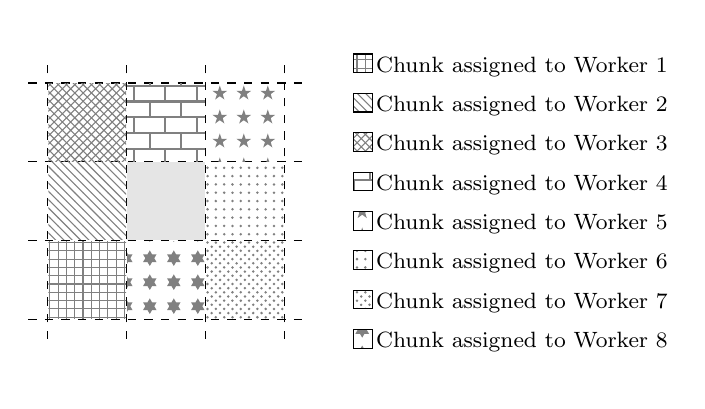
\begin{tikzpicture}[every node/.style={minimum size=1cm-\pgflinewidth, outer sep=0pt}]
    % Graphic area
    \draw[step=1cm, color=black, dashed] (-1.25,-1.25) grid (2.25,2.25);
    \node[fill=gray!20] at (0.5, 0.5) {};
    \node[pattern = bricks, pattern color = gray] at (0.5, 1.5) {};
    \node[pattern = sixpointed stars, pattern color = gray] at (0.5, -0.5) {};
    \node[pattern = fivepointed stars, pattern color = gray] at (1.5, 1.5) {};
    \node[pattern = crosshatch dots, pattern color = gray] at (1.5, -0.5) {};
    \node[pattern = dots, pattern color = gray] at (1.5, 0.5) {};
    \node[pattern = crosshatch, pattern color = gray] at (-0.5, 1.5) {};
    \node[pattern = grid, pattern color = gray] at (-0.5, -0.5) {};
    \node[pattern = north west lines, pattern color = gray] at (-0.5, 0.5) {};

    % Legend
    \node[pattern = grid, pattern color = gray, draw = black, minimum size=0.25cm-\pgflinewidth] at (3, 2.25) {};
    \node[anchor=west] at (3.05, 2.21) {\footnotesize Chunk assigned to Worker 1};
    \node[pattern = north west lines, pattern color = gray, draw = black, minimum size=0.25cm-\pgflinewidth] at (3, 1.75) {};
    \node[anchor=west] at (3.05, 1.71) {\footnotesize Chunk assigned to Worker 2};
    \node[pattern = crosshatch, pattern color = gray, draw = black, minimum size=0.25cm-\pgflinewidth] at (3, 1.25) {};
    \node[anchor=west] at (3.05, 1.21) {\footnotesize Chunk assigned to Worker 3};
    \node[pattern = bricks, pattern color = gray, draw = black, minimum size=0.25cm-\pgflinewidth] at (3, 0.75) {};
    \node[anchor=west] at (3.05, 0.71) {\footnotesize Chunk assigned to Worker 4};
    \node[pattern = fivepointed stars, pattern color = gray, draw = black, minimum size=0.25cm-\pgflinewidth] at (3, 0.25) {};
    \node[anchor=west] at (3.05, 0.21) {\footnotesize Chunk assigned to Worker 5};
    \node[pattern = dots, pattern color = gray, draw = black, minimum size=0.25cm-\pgflinewidth] at (3, -0.25) {};
    \node[anchor=west] at (3.05, -0.29) {\footnotesize Chunk assigned to Worker 6};
    \node[pattern = crosshatch dots, pattern color =gray, draw = black, minimum size=0.25cm-\pgflinewidth] at (3, -0.75) {};
    \node[anchor=west] at (3.05, -0.79) {\footnotesize Chunk assigned to Worker 7};
    \node[pattern = sixpointed stars, pattern color = gray, draw = black, minimum size=0.25cm-\pgflinewidth] at (3, -1.25) {};
    \node[anchor=west] at (3.05, -1.29) {\footnotesize Chunk assigned to Worker 8};

\end{tikzpicture}
\caption{Data partition for each task performing a \texttt{sync\_clusters}. \label{fig:clust-sync-dp}}
\end{figure}

For each core point in $R_i$ (line $4$ in Algorithm \ref{alg:sync-clusters}) we look for neighbor core points (line $6$) and add their cluster id to the corresponding region in our adjacency mattrix (line $7$).

\begin{algorithm}
  \caption{Builds an adjacency matrix from a region w.r.t its neighbours.\label{alg:sync-clusters}}
  \begin{algorithmic}[1]
    \State @task()
    \Function{sync\_clusters}{$region, sub\_neigh\_data$}
        \State $core\_points \gets \text{get\_core\_points}(region)$
        \ForAll{$point \textbf{ in } core\_points$}
            \State $neigh\_cores \gets \text{get\_core\_points}(sub\_neigh)$
            \If{\text{close}($point, n\_point \textbf{ in } neigh\_cores$)}
                \State $adj\_matrix[point\_id].add(n\_point\_id)$
            \EndIf
        \EndFor
        \State \textbf{return} $adj\_matrix$
    \EndFunction
  \end{algorithmic}
\end{algorithm}

\subsection{Cluster Mapping} \label{subsec:cluster-mapping}
In the previous method we introduced our analogy from clusters to graph, let us in this section define it properly.

Let $\mathcal{G}$ be an undirected graph, $\mathcal{N}$ the set of nodes and $\mathcal{E}$ the set of edges. Let $\lbrace M_1, \dots, M_n \rbrace$, where $M_i \in \lbrace 0,1 \rbrace^{|\mathcal{N}|\times |\mathcal{N}|} \hspace{3pt} \forall i \hspace{3pt} \in \lbrace 1, \dots, n\rbrace $, be a set of incomplete adjacency matrices of $G$ fulfiling \ref{eq-1}.
\begin{equation} \label{eq-1}
    \forall (u, v) \in \mathcal{E}, \exists j \in \lbrace 1, \dots, n \rbrace \text{ : } M_j(u, v) = 1
\end{equation}
By incomplete we mean that, except for $n=1$, generally $M_i \neq AM \hspace{3pt} \forall i \in \lbrace 1, \dots, n \rbrace$ where $AM$ is $\mathcal{G}$'s adjacency matrix.

Let us now state the following problem: \emph{given the set $\lbrace M_1, \dots, M_n \rbrace$ find the connected components of $\mathcal{G}$. I.e find $\lbrace S_1, \dots, S_m \rbrace, \hspace{2pt}  S_i \subset \mathcal{N}$ fulfilling \ref{eq-2}.}
\begin{equation} \label{eq-2}
\begin{split}
    & \forall i \in \lbrace 1, \dots, m \rbrace, \forall u, v \in \mathcal{N} \cap S_i \hspace{2pt} \exists \hspace{2pt} \lbrace e_1, \dots e_s \rbrace \\ 
    & e_j \in \mathcal{E} \text{ , a path connecting $u$ and $v$, and this path} \\
    & \text{ does not exist } \forall v \in \left( \mathcal{N} \cap S_i \right)^C
\end{split}
\end{equation}

This problem can be solved in linear time using a BFS or a DFS \cite{linear-adj}, given that we have $AM$. Our case resembles more to the one of dinamically keeping track of the connected components since we will sequentially process each $M_i$. The S.o.A for this problem uses a Disjoint-Set data structure to do so.

A Disjoint-Set (or Union-Find, Merge-Find set) is a data structure that, exactly, keeps track of the elements of a set of elements partitioned in non-overlapping subsets (connected components). Computationally-wise, adding elements can be done in near-constant time ($\mathcal{O}(\alpha (n))$ where $\alpha(n)$ is the inverse Ackermann function).

We claim now that this problem is equivalent to the one of obtaining the core point clusters given the set of adjacency matrices. Each one corresponding to a region $R_i$. The equivalence holds for the following analogies.
\begin{itemize}
    \item[(i)] $\mathcal{N}$ is the set of all the clusters found in each region $R_i$ stacked together
    \item[(ii)] $n$ (the number of incomplete adjacency matrices) is exactly the number of regions $R_i$
    \item[(iii)] Each matrix $M_i$ contains all the connections found by all the tasks spawned in region $R_i$
\end{itemize}
The nodes in the connected components of the graph are exactly all the clusters that need to be merged and the connected components themselves are the clusters we are looking for. Note that transitivity holds \emph{because} we only considered core points for the clusters.

\subsubsection{Cluster Expansion} \label{cluster_exp}
In method \texttt{expand\_clusters} we label reachable points, that is, Non-core points that are in the $\varepsilon$-neighbourhood of a core point.

After the pre processing performed in the \texttt{partial\_scan} method, non-core points can fall into two different groups:
\begin{itemize}
    \item[(i)] Point $p$ that, when processed, was already close to a core point $q$. Case (ii) in \texttt{partial\_scan}. TB-DBSCAN remembers $q$.
    \item[(ii)] Point $p$ that, when processed, was \emph{not} close to a core point. Case (iii) in \texttt{partial\_scan}. TB-DBSCAN remebers $N_{\varepsilon}(p)$ and knows if know is or is not in the $\varepsilon$-neighbourhood of a core-point.
\end{itemize}

Algorithm \ref{alg:expand-clusters} covers case (i) (line 7), case(ii) (line 6) and lastly updates all the labels according to the clusters yield in the Disjoint-Set (line 13).

\begin{algorithm}
  \caption{Label all the reachanle points within a cluster. \label{alg:expand-clusters}}
  \begin{algorithmic}[1]
    \State @task()
    \Function{expand\_clusters}{$square\_data, mappings$}
        \State \Comment{Reachable points labeling}
        \State $non\_core\_points \gets \text{get\_non\_core}(square\_data)$
        \ForAll{$point \textbf{in} non\_core$}
            \If{$point\_id \text{ points to } core\_point$}
                \State $point\_id \gets core\_point\_id$
            \ElsIf{$point\_id \text{ maps to } core\_point$}
                \State $point\_id \gets core\_point\_id$
            \EndIf
        \EndFor
        \State \Comment{Remap the cluster labels according to the sync}
        \State $square\_data\_id \gets \text{remap}(square\_data\_id, mappings)$
        \State \text{save\_to\_file}$(square\_data)$
    \EndFunction
  \end{algorithmic}
\end{algorithm}

FALTA UN GRAFIC GENERAL

%%%%%%%%%%%%%%%%%%%%%%%%%%%%%%%%%%%%%%%%%%%%%%%%%%%%%%%%%%%%
%%%%%%%%%%%%%%%%%%     EVALUATION       %%%%%%%%%%%%%%%%%%%%
%%%%%%%%%%%%%%%%%%%%%%%%%%%%%%%%%%%%%%%%%%%%%%%%%%%%%%%%%%%%

\section{Evaluation} \label{sec:performance}

% JC: Add a section entry phrase for the evaluation. DONE
% JC: Subsection with the infrastructure (hardware description, software versions, etc.) DONE
% JC: Subsection with the configurations evaluated, as well as the metrics considered for the evaluation.
% JC: Results and explanations of them. If more of one evaluation is performed, divide them into subsections (e.g. performance achieved, scalability experiments, etc.) DONE

This section covers the evaluation of the implementation presented. The first subsection \ref{subsec:infrastructure} covers how was the algorithm implemented and tested. The second subsection \ref{subsec:metrics} gathers all the data collected from the different experiments performed. The last subsection \ref{subsec:critical} provides a critical review on the results, what was expected and what has been achieved.

\subsection{Infrastructure} \label{subsec:infrastructure}

As mentioned before, the algorithm has been implemented fully in Python within the PyCOMPSs framework. COMPSs version is the 2.1 and Python's is the 2.7.13 since COMPSs does not support Python 3.X. To run the program hence, the user must have COMPSs installed, the corresponding Python version and the numeric python library (numpy). The algorithm can be ran both locally and in a cluster, in the project's GitHub repository there is a shell script (\texttt{run.sh}) that contains methods to invoke the DBSCAN both as local host (through \texttt{runcompss} command) and to a queuing system (through \texttt{enqueue\_compss} command). 

The experiments were ran on a cluster located in Barcelona. The \href{https://www.bsc.es/user-support/mn4.php#systemoverview}{Mare Nostrum 4} (MN4) is the fourth generetion of supercomputers located in the \href{https://www.bsc.es}{Barcelona Supercomputing Center - Centro Nacional de Supercomputacion (BSC-CNS)} its current Linpack Rmax Performance is 6.2272 Petaflops and it has been running since early July 2017. It is equipped with 48 racks with 3456 nodes. Each node has two Intel Xeon Platinum chips with 24 processors per unit. COMPSs through its queuing script for clusters, \texttt{enqueue\_compss}, requires each node on exclusivity. Therefore from now on, whenever a node is mentioned it must be considered that no other program is going to be running there besides our execution. Additionally the queuing script incorporates a \texttt{cpus\_per\_node} flag that determines the number of processors running in each node.

\subsection{Runtime Metrics} \label{subsec:metrics}

To evaluate the algorithm's performance for different dataset sizes (all three dimensional but with different number of points) the execution time has been measured. This duration is computed inside the python method using the built-in tools and printed through the standard output. For the same dataset, a batch of executions with different number of workers was performed to test the algorithm's scalability. The input parameters vary between different data sizes but never inside the same batch. All the executions were ran in MN4  with Scratch file system. Results are summarized in Table \ref{performance_table}

\begin{table*}[!t]
\centering
\caption{Performance measured on MN4 without tracing and 16 CPUs per node.}
\label{performance_table}
\begin{tabular*}{\textwidth}{c|cc|cc|cc|cc|cc}
 \textbf{SCRATCH}   & \textbf{NP=16} & \textbf{10k} & \textbf{NP = 16} & \textbf{20k} & \textbf{NP = 32} & \textbf{50k} & \textbf{NP = 32} & \textbf{100k} &  \textbf{NP=32} & \textbf{ 200k}\\ \cline{2-11} 
\textbf{Workers}     & \textbf{Time (sec)}   & \textbf{SUp}   & \textbf{Time (sec)}     & \textbf{SUp}   & \textbf{Time (sec)}     & \textbf{SUp}   & \textbf{Time (sec)}    & \textbf{SUp}    & \textbf{Time (sec)}   & \textbf{SUp} \\ \cline{1-11}
\textbf{1}           & 36.12        & 1.00              & 125.03          & 1.00              & 820.14           & 1.00              & 3160.46          & 1.00  &   15030.99 & 1.00          \\
\textbf{2}           & 22.47          & 1.63           & 71.66            & 1.74           & 423.36           & 1.93           & 1623.92          & 1.94 & 7659.83 & 1.96        \\
\textbf{3}           & 18.05          & 2.02           & 55.04           & 2.27           & 308.014          & 2.62           & 1165.10         & 2.71 & 4547.23 & 3.3           \\
\textbf{4}           & 15.91         & 2.25           & 45.60           & 2.74           & 249.59           & 3.28           & 910.30            & 3.47   & 3634.97 & 4.13        \\
\textbf{5}           & 15.01          & 2.40           & 42.49           & 2.94           & 227.93           & 3.59           & 777.19          & 4.06  & 3134.47 & 4.79         \\
\textbf{6}           & 14.55          & 2.48           & 40.23            & 3.16           & 196.69           & 4.16           & 703.90            & 4.48 & 2736.65 & 5.49           \\
\textbf{7}           & 14.3           & 2.52           & 36.36           & 3.43           & 184.00              & 4.45           & 620.53          & 5.09 & 2557.32 & 5.87           \\
\textbf{8}           & 13.64         & 2.64           & 33.61           & 3.72           & 171.00              & 4.79           & 609.21          & 5.18 & 2376.56 & 6.32           \\
\textbf{16}          & 13.45          & 2.68           & 29.02           & 4.30           & 143.00              & 5.73           & 433.12          & 7.29 & 1565.82 & 9.59           \\ \cline{1-11}
\textbf{Seq} & 4690.80         &                & ---              &                & ---              &                & ---              & & --- &                
\end{tabular*}
\end{table*}

\begin{figure}[h!]
\centering	
\begin{tikzpicture}
\begin{axis}[
height=2in,
width=3.5in,
    scaled x ticks = false,
    xlabel = {\# Workers},
    grid = major,
    ylabel = {Speed Up},
    legend entries={10k, 20k, 50k, 100k, 200k}, legend style={at={(0.05,-0.25)},anchor=north west, draw=none, legend columns=-1}
    %xtick={0.028503, 0.0427553,0.0570},
    %xticklabels={$l-2\lambda$, $l-\lambda$,$l$},
    %ytick={0,1,2},
    %yticklabels={0,$|E_{0i}|$,$2|E_{0i}|$},
]
\addplot[mark=o, thick, blue] table {data/10k.dat};
\addplot[mark=o, thick, orange] table {data/20k.dat};
\addplot[mark=o, thick, red] table {data/50k.dat};
\addplot[mark=o, thick, green] table {data/100k.dat};
\addplot[mark=o, thick, purple] table {data/200k.dat};
%Here the blue parabloa is defined
\end{axis}
\end{tikzpicture}
\caption{Speed Up as a function of the number of workers for different datasets.}
\label{speed_up}
\end{figure}

In figure \ref{speed_up} there is a speed up vs number of workers plot. To understand why it increases as the number of points increases check section \ref{q_coi_passa}. Additionally, a runtime vs number of workers plot can be found at \ref{rt_plot}.

\begin{figure}[h!]
\centering	
\begin{tikzpicture}
\begin{axis}[
height=2in,
width=3.5in,
    scaled x ticks = false,
    xlabel = {\# Workers},
    grid = major,
    ylabel = {Execution Time (sec)},
    legend entries={10k, 20k, 50k, 100k, 200k}, legend style={at={(0.05,-0.25)},anchor=north west, draw=none, legend columns=-1}
    %xtick={0.028503, 0.0427553,0.0570},
    %xticklabels={$l-2\lambda$, $l-\lambda$,$l$},
    %ytick={0,1,2},
    %yticklabels={0,$|E_{0i}|$,$2|E_{0i}|$},
]
\addplot[mark=o, thick, blue] table {data/10kRT.dat};
\addplot[mark=o, thick, orange] table {data/20kRT.dat};
\addplot[mark=o, thick, red] table {data/50kRT.dat};
\addplot[mark=o, thick, green] table {data/100kRT.dat};
\addplot[mark=o, thick, purple] table {data/200kRT.dat};
%Here the blue parabloa is defined
\end{axis}
\end{tikzpicture}
\caption{Execution time as a function of the number of workers for different datasets.}
\label{rt_plot}
\end{figure}

\subsection{Critical Analysis} \label{subsec:critical}

\subsubsection{Dependence on the scale parameters:}

From the explanation in Section  it is easy to see that the paradigm has shifted from a two parameter algorithm to a four one. In the one hand this enables, when run by someone familiar to it, the algorithm to adapt better to mutable resources and data loads. In the other hand this also increases the variability of the performance, may be a drawback at some points and makes the implementation not 100\% structure-unaware.

Emphasizing on this two extra parameters, one of them has not got a clear impact on the runtime metrics. The number of comparisons executed by a worker, \texttt{numComp} will determine a certain type of task's length but won't increase their variability. However, \texttt{numParts} chunks the data again having a direct effect on the number of clusters initially found and consequently on the number of tasks performed at the syncing stage. In addition to that, it reduces the average task duration and at the same time makes tasks less homogeneous. This process causes bigger executions' (more points and assigned nodes) behavior more volatile. In spite of that, this scale parameter is necessary to ensure the algorithm's scalability, otherwise it would depend entirely on the data distribution.


To dig in this sections where the algorithm is not performing as expected, or at least not as desired, we undergo a performance analysis using tracing (\href{https://tools.bsc.es/paraver}{Paraver}). In Figure  there is an example of a small execution with  $\texttt{numParts}=16$ (relatively small value of the parameter) and 10000 points. Consequently with the above lines a homogeneous trace is obtained. In Figure  the opposite behavior is exposed. For this second execution the number of points was around 20000 and $\texttt{numParts}=32$. It is easy to see that tasks durations become much more unstable (green flags indicate a task's beginning and ending) and they are not so easily scheduled by the COMPSs runtime.


\subsubsection{On memory, CPUs per node and scalability:} \label{q_coi_passa}

Another issue faced when testing the algorithm is the memory vs cpu per node paradigm. Initially each node has 2GB of RAM, however if the user requests less CPUs per node and exclusivity each worker will virtually have more random access memory since the whole batch is divided between the running threads. When the dataset tends to get bigger and bigger, the memory requested increases as well. Hence the performance at some points might be better with less \texttt{cpus\_per\_node} in spite of the time lost with inter-node communication. To dig deeper into this situation, another set of tests is performed. Results are summarized in Table \ref{cpusComparison}. The \texttt{cpus\_per\_node} values to be compared are 16 and 48. 48 is 16 times 3, therefore to perform a fair comparison the number of workers assigned to the 16 \texttt{cpus\_per\_node} test must be three times the ones assigned to the 48 \texttt{cpus\_per\_node} one. Surprisingly enough given the reasoning above, results do not show a clear dominance of 16 CPUs per node tests over 48 CPUs ones with small datasets. As the size of the input grows and as more calculations are required, the performance is the predicted and 16 \texttt{cpus\_per\_node} tests are quicker.

\subsubsection{On time complexity}

Figures \ref{timeComplexity1} and \ref{timeComplexity2} plot the evolution of the execution time as a function of the size of the input, i.e the number of points, for a fixed number of working nodes and two different \texttt{cpus\_per\_node} parameters, 16 and 48 respectively. \ref{q_coi_passa} shows that there is no evident difference between the two options, as a consequence both Figures look really similar. The main conclusion one can deduce is that, the higher the number of workers (or CPUs in general) the least the application behaves quadratically as its naive sequential implementation and the better PyCOMPSs performs.

\subsubsection{Testing with real data and comparing with S.o.A implementations}

All the previous tests have been performed with synthetic data. The application must as well prove to be useful in real-life applications and when compared to other implementations. A real case use is the one presented in \cite{toolsDBSCAN} where clustering is applied to an app trace to "outline the different trends of the CPU computation areas of parallel applications". Within the same paper, an implementation of the DBSCAN is proposed and thus we will be able to compare both performances. The trace used is one corresponding to:

%%%%%%%%%%%%%%%%%%%%%%%%%%%%%%%%%%%%%%%%%%%%%%%%%%%%%%%%%%%%
%%%%%%%%%%%%%%%%%       CONCLUSIONS     %%%%%%%%%%%%%%%%%%%%
%%%%%%%%%%%%%%%%%%%%%%%%%%%%%%%%%%%%%%%%%%%%%%%%%%%%%%%%%%%%


\section{Conclusion} \label{sec:conclusion}

% Conclusions structure:
% - Describe the achievements of the work (DBSCAN parallelization, performance results, etc.)
% - Considerations (if any).
% - Future work.
%
% JC: There shouldn't be tables of results nor graphs in this section. They should be in the evaluation section.
% JC: I wouldn't divide it in subsections.

Following along the reasoning from \ref{subsec:critical}, the algorithm is really sensitive to changes in the input parameters. Thus this parameters should somehow depend on the resources available, however that would make the algorithm not structure-unaware. This might be one of the reasons why scalability and speed up is not exactly as desired since all the tests for the same dataset are performed under the same input parameters (to be able to compare them). Therefore the measured speedup might be worse in comparison to if we were to run the algorithm manually test by test. 

\begin{table*}[!ht]
\centering
\caption{Execution time comparison with the same number of CPUs but different number of workers and different CPUs per node. Time measured in seconds.}
\label{cpusComparison}
\begin{tabular*}{.95\textwidth}{c|cc|cc|cc|cc|cc}
\textbf{Comparison CPUS per Node} & \multicolumn{2}{c|}{\textbf{10k}} & \multicolumn{2}{c|}{\textbf{20k}} & \multicolumn{2}{c|}{\textbf{50k}} & \multicolumn{2}{c|}{\textbf{100k}} &
\multicolumn{2}{c}{\textbf{200k}}
\\ \hline
\textbf{\#Workers - 16 (48)}      & \textbf{16}     & \textbf{48}     & \textbf{16}     & \textbf{48}     & \textbf{16}     & \textbf{48}     & \textbf{16}      & \textbf{48}   & \textbf{16}     & \textbf{48}  \\ \hline
\textbf{3 (1)}                    & 23.44           & 21.81           & 68.22           & 63.6            & 375.47          & 366.49          & 1326.732         & 1322.73  & 5308.99 & 5501.241035    \\
\textbf{6 (2)}                    & 16.74           & 16.94           & 46.15           & 44.62           & 233.71          & 230.68          & 790.97           & 785.68   & 3205.49 & 3412.54       \\
\textbf{9 (3)}                    & 16.609          & 16.42           & 39.71           & 37.77           & 190.39          & 186.69          & 623.78           & 627.52   & 2427.87 & 2451.26       \\
\textbf{12 (4)}                   & 17.78           & 15.74           & 34.43           & 36.01           & 167.83          & 173.65          & 555.06           & 544.66    & 2039.61 & 2012.89      \\
\textbf{15 (5)}                   & 17.23           & 16.92           & 33.71           & 33.177          & 163.87          & 158.08          & 487.01           & 480.03     & 1707.57 & 1842.83     \\
\textbf{18 (6)}                   & 16.76           & 15.63           & 33.166          & 33.84           & 156.11          & 149.75          & 461.73           & 446.91   & 1486.20 & 1708.76      
\end{tabular*}
\end{table*}

\begin{figure}[t]
\centering
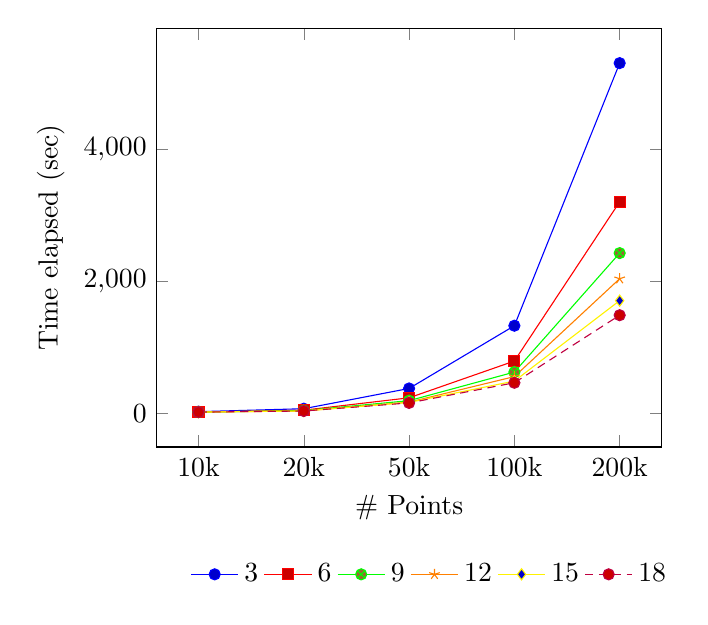
\begin{tikzpicture}
    \begin{axis}
        [
        ,width=8cm
        ,xlabel=\# Points
        ,ylabel=Time elapsed (sec)
        ,xtick=data,
       %,xtick={0,1,...,3}
        ,xticklabels={10k,20k,50k,100k, 200k}
        ,legend entries={3, 6, 9, 12, 15, 18}, legend style={at={(0.05,-0.25)},anchor=north west, draw=none, legend columns=-1}
        ]
        \addplot+[sharp plot] coordinates
        {(0,23.44) (1,68.22) (2,375.47) (3,1326.73) (4, 5308.99)};
        \addplot+[sharp plot, red] coordinates
        {(0,16.74) (1,46.15) (2,233.71) (3,790.97) (4, 3205.49)};
        \addplot+[sharp plot, green] coordinates
        {(0,16.609) (1,39.71) (2,190.39) (3,623.78) (4, 2427.87)};
        \addplot+[sharp plot, orange] coordinates
        {(0,17.78) (1,34.43) (2,167.83) (3,555.06) (4, 2039.61)};
        \addplot+[sharp plot, yellow] coordinates
        {(0,17.23) (1,33.43) (2,163.87) (3,487.01) (4, 1707.57)};
        \addplot+[sharp plot, purple] coordinates
        {(0,16.76) (1,33.16) (2,156.11) (3, 461.73) (4, 1486.2)};
    \end{axis}
\end{tikzpicture}
\caption{Evolution of time elapsed with a fixed number of workers. 16 CPUs per node. \label{timeComplexity1}}
\end{figure}

\begin{figure}[t]
\centering
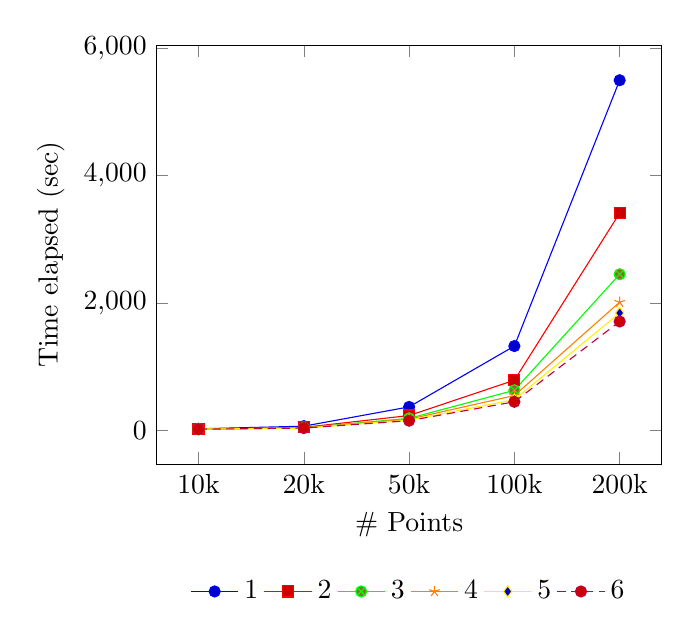
\begin{tikzpicture}
    \begin{axis}
        [
        ,width=8cm
        ,xlabel=\# Points
        ,ylabel=Time elapsed (sec)
        ,xtick=data,
       %,xtick={0,1,...,3}
        ,xticklabels={10k,20k,50k,100k, 200k}
        ,legend entries={1, 2, 3, 4, 5, 6}, legend style={at={(0.05,-0.25)},anchor=north west, draw=none, legend columns=-1}
        ]
        \addplot+[sharp plot] coordinates
        {(0,21.81) (1,63.6) (2,366.49) (3,1322.73) (4, 5501.24)};
        \addplot+[sharp plot, red] coordinates
        {(0,16.94) (1,44.62) (2,230.68) (3,785.68) (4, 3412.54)};
        \addplot+[sharp plot, green] coordinates
        {(0,16.42) (1,37.77) (2,186.69) (3,627.52) (4, 2451.26)};
        \addplot+[sharp plot, orange] coordinates
        {(0,15.74) (1,36.01) (2,173.83) (3,544.66) (4, 2012.89)};
        \addplot+[sharp plot, yellow] coordinates
        {(0,16.92) (1,33.17) (2,158.08) (3,480.03) (4, 1842.83)};
        \addplot+[sharp plot, purple] coordinates
        {(0,15.63) (1,33.84) (2,149.75) (3, 446.91) (4, 1708.76) };
    \end{axis}
\end{tikzpicture}
\caption{Evolution of time elapsed with a fixed number of workers. 48 CPUs per node.} \label{timeComplexity2}
\end{figure}

\subsection{Further Development and Improvement Proposals} \label{further_development}
The main development recommended would be performing a smart guess at execution time of the scale parameters. Empirically it has been proven that if the user is able to choose the right parameters, the algorithm is going to have a great performance. As a consequence, being able to guess them at execution time would guarantee a stability that for this moment can not be ensured.

Secondly, the DBSCAN method could be expanded to a generalized DBSCAN to detect arbitrary cluster densities removing the dependencies to the input parameters, \texttt{minPoints} and $\varepsilon$.

Lastly and in the opposite direction of the second proposal, some research into parallel optimization models so to guess the input parameters (rather than using a thumb rule) could be done.

%%%%%%%%%%%%%%%%%%%%%%%%%%%%%%%%%%%%%%%%%%%%%%%%%%%%%%%%%%%%
%%%%%%%%%%%%%%       ACKNOWLEDGEMENTS     %%%%%%%%%%%%%%%%%%
%%%%%%%%%%%%%%%%%%%%%%%%%%%%%%%%%%%%%%%%%%%%%%%%%%%%%%%%%%%%


\section*{Acknowledgements}

Acks

% JC: In this section we will include the acknowledgements required. Don't worry about it by now. It will be just a paragraph with some references to projects and funding.

%%%%%%%%%%%%%%%%%%%%%%%%%%%%%%%%%%%%%%%%%%%%%%%%%%%%%%%%%%%%
%%%%%%%%%%%%%%%%%       BIBLIOGRAPHY     %%%%%%%%%%%%%%%%%%%
%%%%%%%%%%%%%%%%%%%%%%%%%%%%%%%%%%%%%%%%%%%%%%%%%%%%%%%%%%%%


\begin{thebibliography}{1}
\bibitem{compss}
Badia, R. M., J. Conejero, C. Diaz, J. Ejarque, D. Lezzi, F. Lordan, C. Ramon-Cortes, and R. Sirvent \textit{COMP Superscalar, an interoperable programming framework} SoftwareX, Volumes 3–4, Pages 32–36, (2015)
\bibitem{related_1}
D. Arlia and M. Coppola, \textit{Experiments in Parallel Clustering
with DBSCAN} in Euro-Par Springer, LNCS, 2001, pp.
326-331.(2001)
\bibitem{related_2}
 S. Brecheisen et al., \textit{Parallel Density-Based Clustering of Complex Objects} Advances in Knowledge Discovery and
Data Mining, pp. 179-188 (2006)
\bibitem{related_3}
Yaobin He et al. \textit{MR-DBSCAN: a scalable MapReduce-based DBSCAN algorithm for heavily skewed data} Frontiers of Computer Science, vol 8, no. 1, pp 83-99, (2014)
\bibitem{related_4}
Md. Mostofa Ali Patwary et al. \textit{A new scalable parallel DBSCAN algorithm using the disjoint-set data structure} Conference: High Performance Computing, Networking, Storage and Analysis (SC), (2012)
\bibitem{related_5}
Alessandro Lulli, Matteo Dell'Amico, Pietro Michiardi, Laura Ricci \textit{NG-DBSCAN: scalable density-based clustering for arbitrary data}. Proceedings of the VLDB Endowment Volume 10 Issue 3, p. 157-168 (2016)
\bibitem{original-paper}
Ester, Martin Kriegel, Hans-Peter Sander, Jorg Xu, Xiaowei \textit{A density-based algorithm for discovering clusters in large spatial databases with noise.} Proceedings of the Second International Conference on Knowledge Discovery and Data Mining (KDD-96) (1996)
\bibitem{kmeans}
MacQueen, J. B. \textit{Some Methods for classification and Analysis of Multivariate Observations.} Proceedings of 5th Berkeley Symposium on Mathematical Statistics and Probability. (1967)
\bibitem{pycompss}
Enric Tejedor, Yolanda Becerra, Guillem Alomar, Anna Queralt, Rosa M. Badia, Jordi Torres, Toni Cortes, Jesús Labarta, \textit{PyCOMPSs: Parallel computational workflows in Python}  IJHPCA 31(1): 66-82 (2017)
\bibitem{toolsDBSCAN}
J. Gonzalez, J. Gimenez, J. Labarta. \textit{Automatic detection of parallel applications computation phases}.
\bibitem{linear-adj}
    Hopcroft, J., Tarjan, R. \textit{Algorithm 447: efficient algorithms for graph manipulation} Communications of the ACM, 16 (6): 372–378 (1973)
\end{thebibliography}


\end{document}


